
 Из системы уравнение Максвелла получим следующее волновое уравнение (\ref{sec:wave_equation}):

\begin{equation}
 \Laplace \vec{E} - k_0^2 \vec{D} = \Laplace \vec{E} - k_0^2 (1+\chi)\vec{E} = 0
 \label{eq:wave_maxwel}
\end{equation}
\noindent
Как было упомянуто выше, в кристалле распространяются две волны:
\begin{equation}
 \begin{cases}
   \vec{E}_0 = \vec{e}_0 E_0 e^{i\vec{q}_0\vec{r}}
   \\
   \vec{E}_h = \vec{e}_h E_h e^{i\vec{q}_h\vec{r}}
 \end{cases}
 \label{eq:E_0_E_h}
\end{equation}
\noindent
где произведение единичных векторов $\vec{e}_0$ и $\vec{e}_h$:
\begin{equation}
\vec{e}_0 \cdot \vec{e}_h = C
 \begin{cases}
   1, \quad \quad \quad \quad  \sigma    - \text{поляризация}\\
   \cos(2\theta_B), \quad   \pi - \text{поляризация}
 \end{cases}
\end{equation}

\begin{figure}[H]
  \centering
  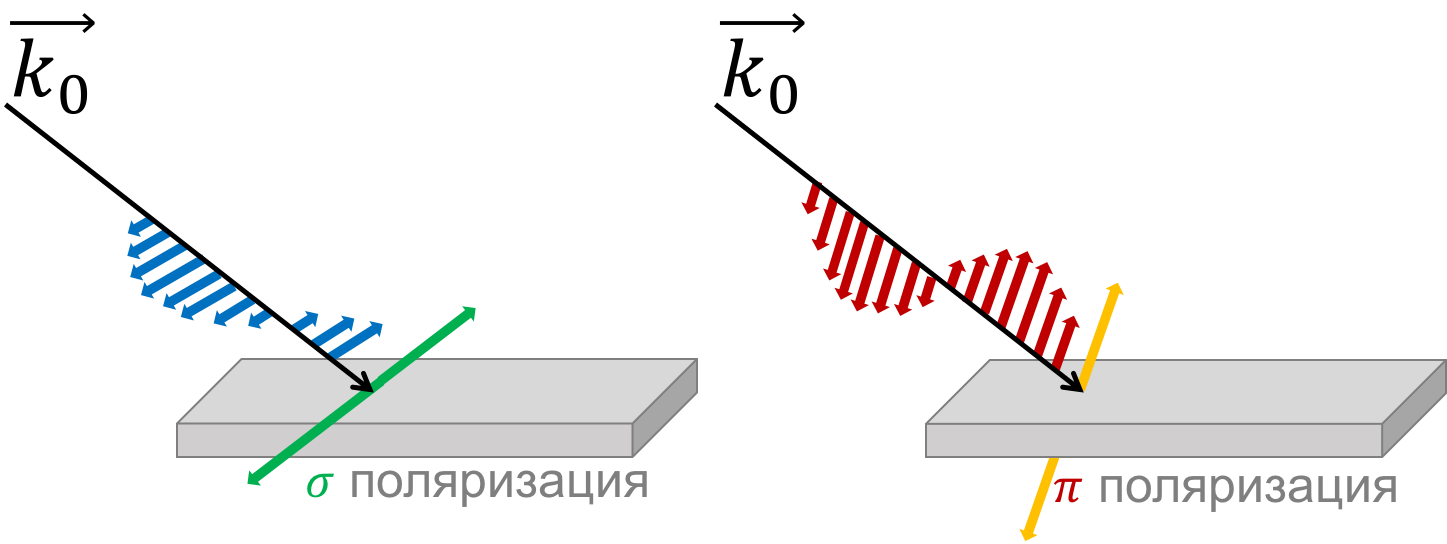
\includegraphics[width=0.7\textwidth]{images/polarize_E.png}
  \caption{ Колебание вектора напряженности электрического поля для разных типов линейной поляризации рентгеновского излучения}
  \label{ris:polarize_E}
\end{figure}

Подставим (\ref{eq:E_0_E_h}) в уравнение (\ref{eq:wave_maxwel}) и получим
систему динамических уравнений:
\begin{equation}
 \begin{cases}
   \delta_0 E_0 - C\chi_{-h}E_h=0
   \\
   \delta_h E_h - C\chi_{h}E_0=0
 \end{cases}
\end{equation}
\noindent
где,
\begin{equation}
   \delta_{(0,h)} = \frac{q_{(0,h)}^2}{k_0^2}-1-\chi_0
\end{equation}

Прировняем детерминант системы к 0, получив при этом дисперсионное уравнение следующего вида:

\begin{equation}
   \delta_0 \delta_h -C^2 \chi_h \chi_{-h} = 0
\end{equation}

Воспользуемся равенством тангенциальных компонент волнового вектора при переходе между средами (\ref{eq:k_h_squred}, \ref{eq:k_0_squred}),
необходимо отметить $k_h == q_h$ - т.к при выходе излучения из среды происходит лишь преломление, суммарная интенсивность останется прежней.
\begin{equation}
 \begin{cases}
   \delta_0 = \frac{q_0^2 - k_0^2}{k_0^2} - \chi_0 = 2\varepsilon\gamma_0 - \chi_0
   \\
   \delta_h = \frac{q_h^2 - k_0^2}{k_0^2} - \chi_0 = 2\varepsilon\gamma_h - \alpha \chi_0
 \end{cases}
\end{equation}
\noindent
где $\alpha$ соответствует выражению (\ref{eq:alpha}). Дисперсионное уравнение с учетом граничных условий
следущий вид:

\begin{equation}
   (2\varepsilon \gamma_0 - \chi_0)(2\varepsilon \gamma_h - \alpha - \chi_0) - C^2 \chi_h\chi_{-h} = 0
\end{equation}

Решив уравнение относительно параметра аккомодации $\varepsilon$ получим два корня:

\begin{equation}
   \varepsilon_{1,2} = \frac{1}{4\gamma_0} \left( \chi_0 (1-b) - b\alpha \pm \left( [\chi_0(1+b)+b\alpha]^2 - 4bC^2 \cdot \chi_{h}\chi_{-h} \right)^{1/2} \right)
\end{equation}
\noindent
где b - соответсвует (\ref{eq:koef_b}),  а произведение коэффициентов поляризуемости:
 $$\chi_{h} \cdot \chi_{-h} = Re(\chi_{h})^2-Im(\chi_{h})^2 - 2i \quad Re(\chi_{h}) \cdot Im(\chi_{h})$$

Наличие двух решений говорит о том, что в кристалле имеется две проходящие и две дифрагированные волны, но
анализ полученного решения $ \varepsilon_{1,2}$ показывает что один корень имеет положительную мнимую часть, а второй
отрицательную. Мнимая часть отвечает за поглощение и в случае отрицательно корня волна распространяясь
вглубь кристалла экспоненциально затухает. Поэтому будем выбирать всегда корень с отрицательной мнимой частью
$Im(\varepsilon)>0$.

Амплитудный коэффициент отражение
\begin{equation}
    R = \frac{E_0}{E_h} = \frac{\delta_0}{C\chi_{-h}} = \frac{2\varepsilon\gamma_0-\chi_0}{C\chi_{-h}}
\end{equation}

Кривая диффракционного отражения (КДО) \cite{Bushuev_Oreshko_2002}
\begin{equation}
    \label{eq:KDO_self}
    P (\vartheta) =  |\frac{\gamma_h}{\gamma_0} \cdot R|^2
\end{equation}


\begin{figure}[H]
  \centering
  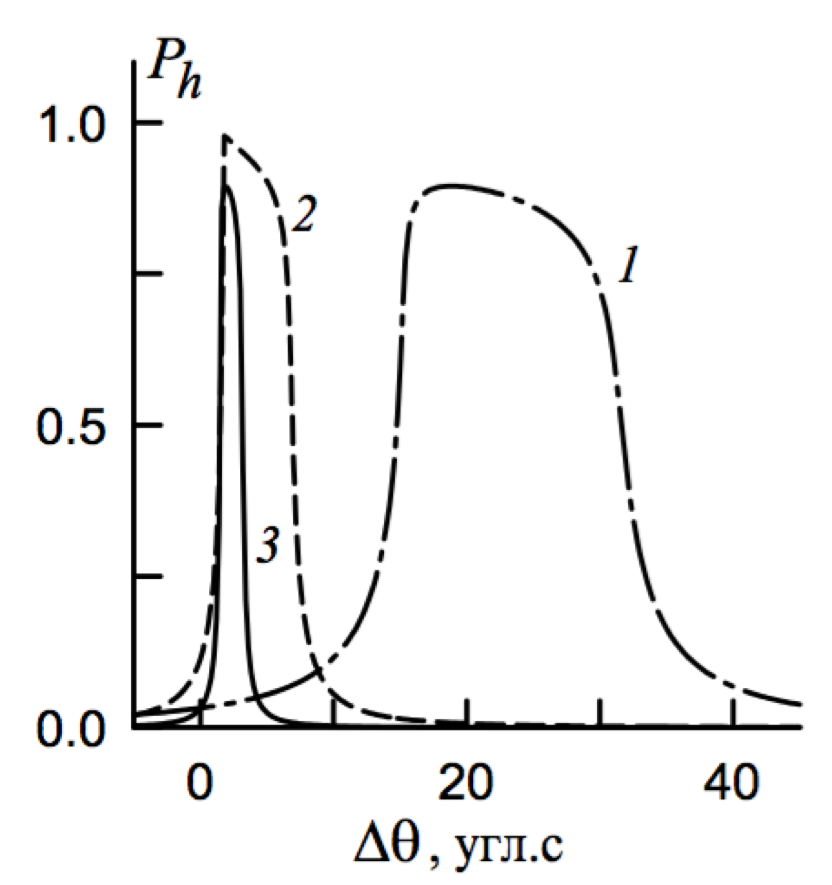
\includegraphics[width=0.5\textwidth]{images/typical_rocking_curve.png}
  \caption{КДО (220) $CuK_{\alpha}$ - излучения от кристалла кремния. Коээфициент ассиметрии
  отражения $b$: кривые 1 - 0.1, 2 - 1, 3 - 10}
  \label{ris:typical_rocking_curve}
\end{figure}

На рис. \ref{ris:typical_rocking_curve} приведен типичный пример собственной кривой дифракционного отражения
для разных коэффициентов асимметрии \cite{Bushuev_Oreshko_2002}.
